\clearpage
\phantomsection

\setcounter{chapter}{1}
\chapter[{ĐÁNH GIÁ ẢNH HƯỞNG CỦA CẤU HÌNH MẢNG ĂNG-TEN TRONG NHẬN DẠNG HỆ THỐNG MIMO KÍCH THƯỚC LỚN}]{Đánh giá ảnh hưởng của cấu hình mảng ăng-ten trong nhận dạng hệ thống MIMO kích thước lớn}
\label{sec:CRB}

Trong chương này, tác giả sẽ xem xét sự ảnh hưởng của các cấu hình mảng ăng-ten khác nhau đến sai số của việc ước lượng kênh truyền trong các hệ thống mMIMO. Đầu tiên, mô hình kênh truyền có cấu trúc cho hai cấu hình mảng ăng-ten 1D và 3D sẽ được giới thiệu. Sau đó là trình bày về việc sử dụng CRB để ước lượng sai số trong các bộ nhận dạng sử dụng pilot và SB. Các kết quả mô phỏng được đưa ra để cho thấy hiệu quả của mô hình kênh truyền có cấu trúc, mảng ăng-ten 3D (UCyA), và phương pháp ước lượng SB trong việc nhận dạng hệ thống viễn thông.

\section{Mô hình kênh truyền có cấu trúc với các cấu hình mảng ăng-ten khác nhau}\label{SM}

Mô hình toán học của một hệ thống mMIMO sử dụng điều chế ghép kênh phân chia theo tần số trực giao (OFDM - Orthogonal Frequency-division Multiplexing) với $K$ sóng mang con trong kênh đường lên gồm $T$ ăng-ten phát và $L$ ăng-ten thu (giả thiết các ăng-ten là vô hướng). Mỗi ký hiệu OFDM bao gồm $K$ ký hiệu dữ liệu và một phần tiền tố vòng (CP - Cyclic Prefix). Giả sử độ dài của CP lớn hơn hoặc bằng thời gian trễ tối đa của kênh truyền (coherent time). Tại ăng-ten thu thứ $l$, sau khi đã loại bỏ thành phần CP và thực hiện biến đổi Fourier (FFT - Fast Fourier Transform), tín hiệu đầu ra tại ăng-ten thu thứ $l$ ($\mathbf{x}_l$) được biểu diễn như sau~\cite{Ladaycia2017}:
\begin{equation}
    \mathbf{x}_{l}=\sum_{t=0}^{T-1} \mathcal{F} \mathcal{T}\left(h_{l, t}\right) \frac{\mathcal{F}}{K} \mathbf{s}_{j}+\mathbf{w}_{l}
\end{equation}
trong đó $\mathcal{F}$ đại diện cho ma trận Fourier rời rạc, gồm $K$ điểm và $\mathcal{T}$ là ma trận lặp lại của $h_{l, t}$. Tiếp đến, $\mathbf{s}_{j}$ là ký hiệu OFDM thứ $k$ có độ dài $K$ và $\mathbf{w}_{l} \in \mathbb{C}^{K \times 1}$ là tạp âm AWGN có dạng i.i.d phân bố Gauss $\mathcal{C} \mathcal{N}\left({0}, \sigma_{\mathbf{w}}^{2} \mathbf{I}_L\right)$. 
Cuối cùng, $h_{l, t}$ là hệ số kênh thuộc ma trận kênh truyền được biểu diễn dưới dạng véc-tơ $\mathbf{h} \in \mathbb{C}^{L T \times 1}$.
\begin{equation}
    \label{eq:1}
    \begin{aligned} 
        \mathbf{h} &=\left[\mathbf{h}_{0}^{\top}, \mathbf{h}_{1}^{\top}, \ldots, \mathbf{h}_{L - 1 }^{\top}\right]^{\top}, \\ \mathbf{h}_{l} &=\left[h_{l, 0}, h_{l, 1}, \ldots, h_{l, T - 1 }\right]^{\top}
    \end{aligned}
\end{equation}
Giả sử rằng $M$ là số lượng đường truyền giữa một cặp ăng-ten phát, thu. Dựa trên hướng tiếp cận mô hình kênh truyền có cấu trúc, $h_{l, t}$ được mô hình tương ứng với $M$ đường truyền, mỗi đường truyền bao gồm hệ số khuếch đại phức và véc-tơ lái ($\varphi$ - steering) như sau:
\begin{equation}
\label{eq:2}
    % \begin{aligned}
        h_{l, t} = \sum\limits_{m=0}^{M-1} \beta_{m, t} e^{\varphi_{m, t}} = \sum\limits_{m=0}^{M-1} \beta_{m, t} \cdot e^{-i k_s c_l(\theta_{m, t}, \phi_{m, t})} 
    % \end{aligned}
\end{equation}
tại tia thứ $m$, hệ số $\beta$ biểu diễn cho hệ số khuếch đại phức. Góc ngẩng và góc phương vị của hướng sóng đến (DoA)\footnote{Để đơn giản hoá, thông tin về DoD được coi là không biết trước tại bên thu của kênh đường lên.} lần lượt là  $\theta$, $\phi$. Các ký hiệu còn lại trong phương trình~(\ref{eq:2}) lần lượt là:
\begin{equation}
    \begin{aligned}
        &k_s = 2\pi/\lambda \\
        &c_l(\theta_{m, t}, \phi_{m, t}) = \widehat{\boldsymbol{c}} \cdot \boldsymbol{c}_l \\
        &\widehat{\boldsymbol{c}}=\sin \theta_{m, t} \cos \phi_{m, t} \widehat{\boldsymbol{x}}+\sin \theta_{m, t} \sin \phi_{m, t} \widehat{\boldsymbol{y}}+\cos \theta_{m, t} \widehat{\boldsymbol{z}} \\
        &\boldsymbol{c}_l=x_{l} \widehat{\boldsymbol{x}}+y_{l} \widehat{\boldsymbol{y}}+z_{l} \hat{\boldsymbol{z}}
    \end{aligned}
\end{equation}
trong đó, $\lambda$ là bước sóng; $\widehat{\boldsymbol{c}}$ là véc-tơ đơn vị trong hệ toạ độ đề-các (Descartes) ba chiều của DoA; và $\boldsymbol{c}_l$ là vị trí của phần tử thứ $l$ trong mảng ăng-ten bên thu ứng với toạ độ ($x_l, y_l, z_l$).
\begin{figure}[ht]
    \centering
    \subcaptionbox{Mảng thẳng cách đều}
        [0.49\linewidth]
        {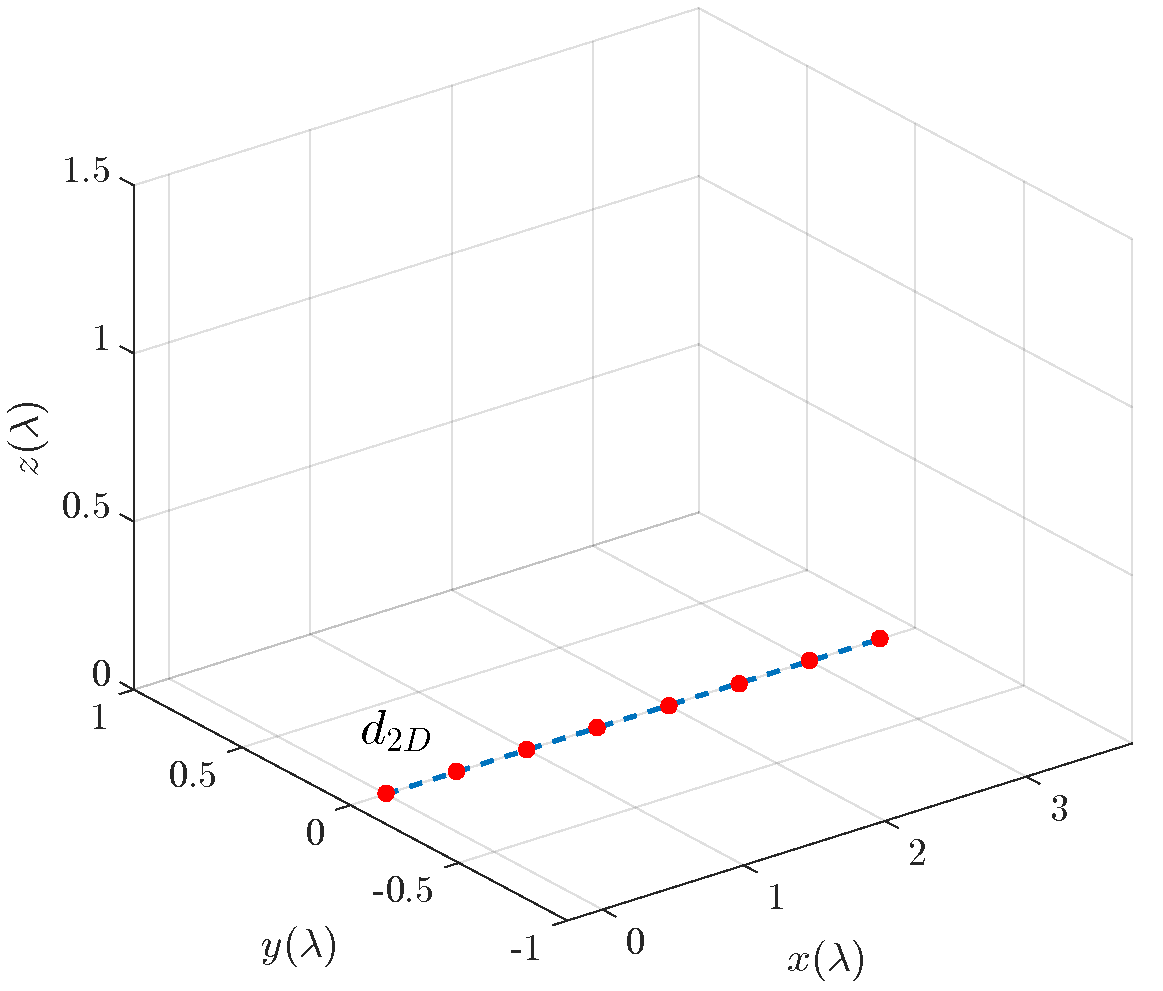
\includegraphics[width=\linewidth]{figures/ULA_2.pdf}}
    \hfill
    \subcaptionbox{Mảng trụ cách đều}
        [0.49\linewidth]
        {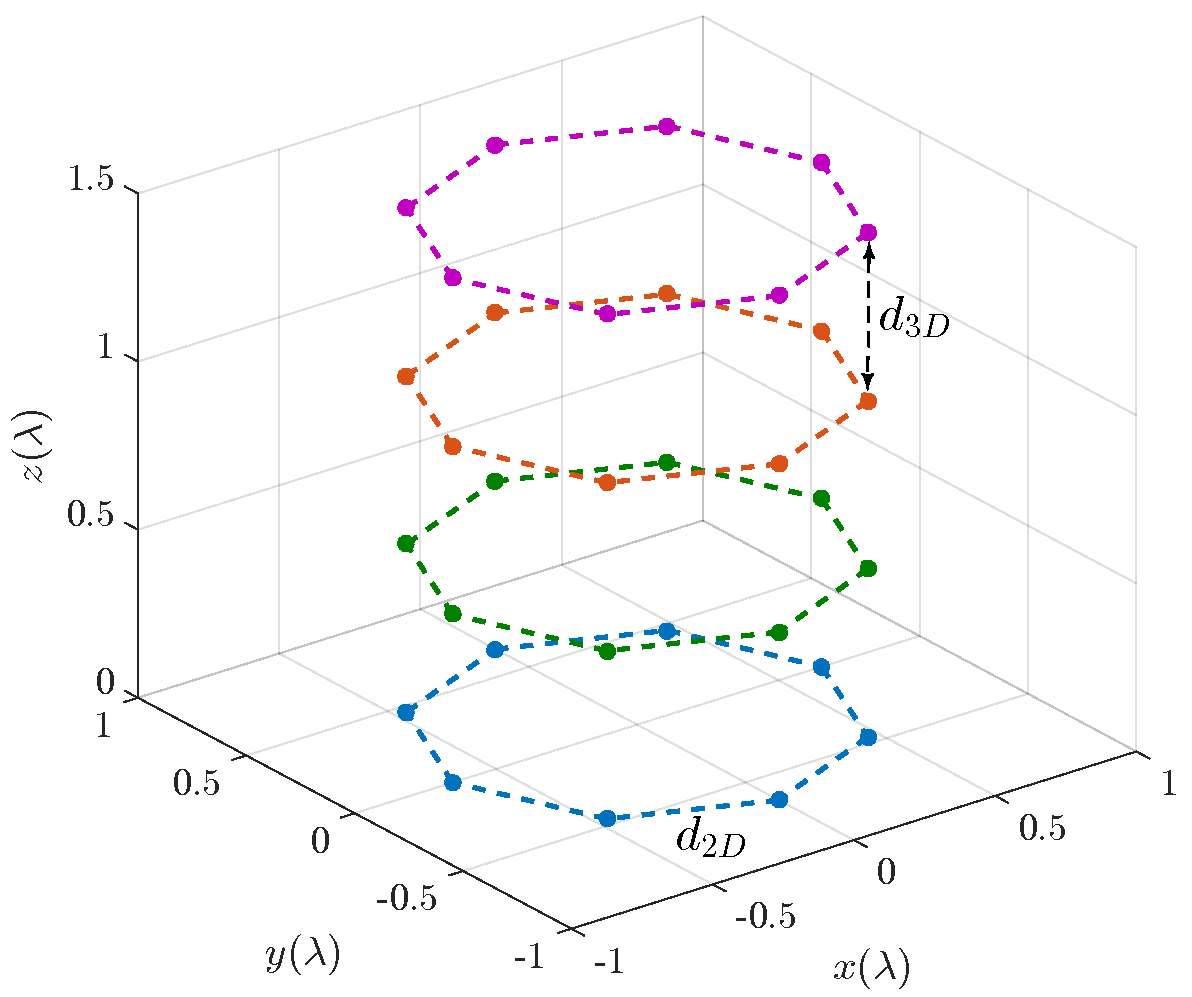
\includegraphics[width=\linewidth]{figures/UCyA_2.pdf}}
    \caption{Minh họa hai cấu hình 1D và 3D của các mảng ăng-ten.}
    \label{fig:antenstruct}
\end{figure}

Hai cấu hình của các mảng ăng-ten mảng thẳng các đều (ULA) và cấu hình mảng trụ cách đều (UCyA), biểu diễn trên hình~\ref{fig:antenstruct}, được khảo sát trong luận văn. Ứng với mảng 1D, ULA là mảng ăng-ten thẳng đơn giản nhất có $N_{ULA}$ phần tử cách đều nhau một khoảng $d_{2D}$. Ứng với mảng ăng-ten 3D, cấu hình UCyA gồm $N_{3D}$ lớp của $N_{UCA}$ phần tử thuộc một mảng tròn cách đều (UCA - Uniform Circle Array) được xem xét. Với khoảng cách giữa các phần tử trong mảng UCA cũng là $d_{2D}$ và khoảng cách giữa các lớp của UCyA là $d_{3D}$ theo hướng dọc trục $z$. Từ đó, bán kính $r$ của mảng vòng UCA được tính như sau:
\begin{equation}
    r = \frac{1/2 \cdot d_{2D}}{\sin(\pi/N_{UCA})}
\end{equation}

Toạ độ ($\boldsymbol{c}_l$) của các phần tử trong hai cấu hình mảng ăng-ten nêu trên là:
\begin{align} 
    &\boldsymbol{c}_l(\text{ULA}) = \;\; \begin{cases}
    x_l = n_{ULA} * d_{2D}\\ 
    y_l = 0\\ 
    z_l = 0
    \end{cases}
    \\
    &\boldsymbol{c}_l(\text{UCyA}) = \begin{cases}
    x_l = r * \sin(n_{UCA} * \frac{2\pi}{N_{UCA}})\\ 
    y_l = r * \cos(n_{UCA} * \frac{2\pi}{N_{UCA}})\\ 
    z_l = n_{3D} * d_{3D}
    \end{cases}
\end{align}
với $n_{ULA} = 0, 1, \ldots, N_{ULA}-1$; $n_{UCA} = 0, 1, \ldots, N_{UCA}-1$, và $n_{3D} = 0, 1, \ldots, N_{3D}-1$.


\section{Đường bao Cramér Rao cho giải thuật nhận dạng hệ thống không mù và bán mù}\label{CRB}

Trong mục này, tác giả sẽ trình bày về phương pháp đánh giá hiệu năng sử dụng CRB cho cả hai mô hình kênh truyền có cấu trúc (structured) và không sử dụng cấu trúc (unstructured) trong các hệ thống mMIMO. Sau đó, so sánh hiệu năng của hệ thống trong các trường hợp: (i) sử dụng pilot (OP - Only Pilot); (ii) bán mù (SB) sử dụng thêm một phần thông tin từ đặc trưng thống kê của dữ liệu, dựa trên đường bao Cramér Rao. 
\subsection{CRB trong trường hợp chỉ sử dụng pilot}

Như trình bày ở phần mở đầu của luận văn, việc sử dụng các ký hiệu pilot hay tín hiệu tham chiếu để ước lượng sự ảnh hưởng của kênh truyền vô tuyến là phương pháp mà WiFi hay 5G đang sử dụng. Về cơ bản, trong các bộ truyền nhận OFDM, $K_p$ ký hiệu pilot sẽ được chèn vào đoạn dữ liệu truyền đi và cả bên thu và phát đều biết trước các giá trị của các ký hiệu pilot này. Bên thu khai thác các ký hiệu pilot thu được để ước lượng kênh truyền, từ đó tính ma trận nghịch đảo để khôi phục lại tín hiệu gốc. Tuy nhiên, chưa có thuật toán nào có thể cho độ chính xác tuyệt đối trong việc nhận dạng kênh truyền vô tuyến thực. Do đó, các chuẩn truyền thông chỉ đưa ra phương pháp là tăng/giảm số lượng pilot khi kênh truyền ở các trạng thái khác nhau. Vậy nên, để so sánh hiệu suất làm việc của các giải thuật, đường bao Cramér Rao~\cite{Kay1993} có thể được sử dụng. 
% Đây là phương pháp được sử dụng rộng rãi để ước lượng độ chính xác tối đa của các bộ nhận dạng không thiên vị (unbias).
CRB cho kết quả là lỗi ước lượng thấp nhất mà một thuật toán ước lượng không lệch có thể đạt được. Đường bao này thường được sử dụng rộng rãi trong các bài toán tối ưu và đánh giá lỗi ước lượng của các thuật toán.
Biểu diễn của CRB như sau:
\begin{equation}
    \text{CRB}(\boldsymbol{\Theta}) = \mathbf{J}_{\boldsymbol{\Theta}\boldsymbol{\Theta}}^{-1}
\end{equation}
trong đó, $\mathbf{J}_{\boldsymbol{\Theta}\boldsymbol{\Theta}}$ là ma trận thông tin Fisher (FIM - Fisher Information Matrix) với $\boldsymbol{\Theta}$ là các véc-tơ tham số không biết trước cần được ước lượng.

\subsubsection*{\textbf{CRB cho mô hình kênh không sử dụng cấu trúc}}
Trong mô hình kênh không sử dụng cấu trúc, $\boldsymbol{\Theta} \simeq	 \mathbf{h}$~\cite{Ladaycia2017}, FIM chỉ phụ thuộc vào các ký hiệu pilot nên sẽ được ký hiệu là $\mathbf{J}_{\boldsymbol{\Theta}\boldsymbol{\Theta}}^p$. Từ đó, các tham số cần được ước lượng sẽ được biểu diễn như sau~\cite{Menni2012}\footnote{Công suất nhiễu được bỏ qua ($\sigma^2_{\mathbf{w}}$) do lỗi ước lượng của tạp âm không ảnh hưởng đến $\mathbf{h}$.}:
\begin{equation}
    \boldsymbol{\Theta}=\left[\mathbf{h}^{\top},  \quad  \left(\mathbf{h}^{*}\right)^{\top}\right]
\end{equation}

Trong các hệ thống mMIMO-OFDM, $K_p$ ký hiệu pilot sẽ được sắp xếp trong các ký hiệu OFDM~\cite{Garro2020} và do giả thiết tạp âm là một quá trình ngẫu nhiên i.i.d., FIM trong trường hợp OP thu được như sau:
\begin{equation}
\label{eq:9}
    \mathbf{J}_{\boldsymbol{\Theta} \boldsymbol{\Theta}}^{p}=\sum_{i=1}^{K_{p}} \mathbf{J}_{\boldsymbol{\Theta} \boldsymbol{\Theta}}^{p_{i}}
\end{equation}
với $\mathbf{J}_{\boldsymbol{\Theta} \boldsymbol{\Theta}}^{p_{i}}$ là FIM tương ứng với pilot thứ $i$~\cite{Kay1993} được cho bởi:
\begin{equation}
    \label{eq:10}
    \begin{aligned}
        \mathbf{J}_{\boldsymbol{\Theta} \boldsymbol{\Theta}}^{p_{i}} &=\mathbb{E}\left\{\left(\frac{\partial \ln p(\mathbf{x}(i), \mathbf{h})}{\partial \boldsymbol{\Theta}^{*}}\right)\left(\frac{\partial \ln p(\mathbf{x}(i), \mathbf{h})}{\partial \boldsymbol{\Theta}^{*}}\right)^{H}\right\} \\
    \end{aligned}
\end{equation}
trong đó $\mathbb{E}$ là toán tử kỳ vọng; $p(\mathbf{x}(i), \mathbf{h})$ là hàm mật độ xác suất (PDF - Probability Density Function) của tín hiệu nhận được đã biết $\mathbf{h}$. Phương trình~(\ref{eq:10}) gồm các phép đạo hàm số phức, nên có thể biểu diễn dưới dạng:
\begin{equation}
    \mathbf{J}_{\boldsymbol{\Theta} \mathbf{\Theta}}^{p_{i}}=\frac{\mathbf{s}(i)^{H} \mathbf{s}(i)}{\sigma_{\mathbf{w}}^{2}}
\end{equation}

\subsubsection*{\textbf{CRB cho mô hình kênh có cấu trúc}}

Mô hình kênh có cấu trúc như trên phương trình~(\ref{eq:2}), các phần tử trong ma trận $\mathbf{H}$ được biểu diễn dưới dạng các tia có hệ số khuếch đại phức, véc-tơ lái khác nhau. Véc-tơ tham có kích thước $4TM~\times 1$ cần được ước lượng là:
\begin{equation}
    \boldsymbol{\Theta}=\left[ \boldsymbol{\beta}^\top, \quad \boldsymbol{(\beta^*)}^\top, \quad \boldsymbol{\theta}^\top, \quad \boldsymbol{\phi}^\top \right]^\top
\end{equation}
với $\boldsymbol{\beta}=\left[\beta_{0,0}, \ldots, \beta_{M-1, T -1}\right]^{\top}$, $\boldsymbol{\beta^*}=\left[\beta^*_{0,0}, \ldots, \beta^*_{M-1, T - 1}\right]^{\top}$, $\boldsymbol{\theta}=\left[\theta_{0,0}, \ldots, \theta_{M-1, T - 1}\right]^{\top}$, và $\boldsymbol{\phi}=\left[\phi_{0,0}, \ldots, \phi_{M-1, T - 1}\right]^{\top}$ lần lượt tương ứng là các véc-tơ có kích thước $TM \times 1$ của hệ số khuếch đại phức, liên hợp phức của hệ số khuếch đại phức, góc ngẩng, và góc phương vị của DoA. Dựa trên phép chuyển đổi của việc đạo hàm theo các tham số kể trên, FIM ($\mathbf{J}^p_{\mathbf{h} \mathbf{h}}$) của kênh truyền $\mathbf{h}$ trên (\ref{eq:1}) sẽ là:
\begin{equation}
\label{eq:13}
    \mathbf{J}^p_{\mathbf{h} \mathbf{h}}=\frac{\partial \mathbf{h}}{\partial \boldsymbol{\Theta}} \mathbf{J}^p_{\boldsymbol{\Theta} \boldsymbol{\Theta}} {\frac{\partial \mathbf{h}}{\partial \boldsymbol{\Theta}}}^{H}
\end{equation}
với 
\begin{equation}
\label{eq:2.15}
    \frac{\partial \mathbf{h}}{\partial \boldsymbol{\Theta}}=
    \left[\frac{\partial \mathbf{h}}{\partial \boldsymbol{\beta}}, 
    \frac{\partial \mathbf{h}}{\partial \boldsymbol{\beta^*}},
    \frac{\partial \mathbf{h}}{\partial \boldsymbol{\theta}}, 
    \frac{\partial \mathbf{h}}{\partial \boldsymbol{\phi}}\right]
\end{equation}
Chi tiết hơn, đạo hàm riêng theo $\boldsymbol{\beta}$ ở phương trình~(\ref{eq:2.15}) có dạng như sau:
\begin{subequations}
    \begin{align}
    &\frac{\partial \mathbf{h}}{\partial \boldsymbol{\beta}}=
    \left[\begin{array}{llll}
        \boldsymbol{B}_{0}^{\top}, & \boldsymbol{B}_{1}^{\top}, & \ldots, & \boldsymbol{B}_{L - 1}^{\top}
    \end{array}\right]^{\top}\\
    &\boldsymbol{B}_{l}=\operatorname{diag}\left(\left[\boldsymbol{B}_{l, 0}, \quad \boldsymbol{B}_{l, 1}, \quad \ldots, \quad \boldsymbol{B}_{l, T - 1}\right]\right) \\
    &\boldsymbol{B}_{l, t}=\left[\begin{array}{cccc}
        \frac{\partial h_{l, t}}{\partial \beta_{0, t}} &
        \frac{\partial h_{l, t}}{\partial \beta_{1, t}} & 
        \ldots & 
        \frac{\partial h_{l, t}}{\partial \beta_{M-1, t}}
    \end{array}\right]^\top
    \end{align}
\end{subequations}
Các đạo hàm riêng của $h_{l, t}$ theo $\beta_{m,t}, \beta^*_{m,t}, \theta_{m, t}, \phi_{m, t}$ được biểu diễn chi tiết trên các phương trình~(\ref{eq:15}).

\begin{subequations}
\label{eq:15}
    \begin{align}
    &\frac{\partial h_{l, t}}{\partial \beta_{m, t}}= \frac{1}{2} (1 - i) \cdot e^{-i k_s c_l(\theta_{m, t}, \phi_{m, t})} &  \\
    &\frac{\partial h_{l, t}}{\partial \beta^*_{m, t}}= \frac{1}{2} (1 + i) \cdot e^{-i k_s c_l(\theta_{m, t}, \phi_{m, t})} \\
    &\frac{\partial h_{l, t}}{\partial \theta_{m, t}}=
    \beta_{m, t} 
    [-i k_s (\cos\theta_{m, t} \cos\phi_{m, t} x_l + \cos\theta_{m, t} \sin\phi_{m, t} y_l
    - \sin \theta_{m, t} z_l)] \cdot e^{-j k_s c_l(\theta_{m, t}, \phi_{m, t})} \\ 
    &
    \frac{\partial h_{l, t}}{\partial \phi_{m, t}}=\beta_{m, t}
     [-i k_s (-\sin\theta_{m, t} \sin\phi_{m, t} x_l + \sin\theta_{m, t} \cos\phi_{m, t} y_l 
    + \cos \theta_{m, t} z_l)] \cdot e^{-i k_s c_l(\theta_{m, t}, \phi_{m, t})}
    \end{align}
\end{subequations}
với $i$ tương ứng là đơn vị ảo trong các số phức.

\subsection{CRB trong trường hợp bán mù}

Theo hướng tiếp cận SB, ngoài sử dụng các ký hiệu pilot, các bộ nhận dạng còn sử dụng thêm thông tin từ các ký hiệu dữ liệu (data) không biết trước trong việc ước lượng kênh truyền. Trong phần này, giả thiết rằng các ký hiệu pilot và data trong ký hiệu OFDM là độc lập về mặt thống kê. 

\subsubsection*{\textbf{CRB cho mô hình kênh không sử dụng cấu trúc}}

FIM của phương pháp SB có thể được biểu diễn đơn giản là tổng của FIM từ các ký hiệu pilot và FIM từ các ký hiệu data như dưới đây:
\begin{equation}
    \label{eq:17}
    \mathbf{J}_{\boldsymbol{\Theta} \boldsymbol{\Theta}}^{SB}= \mathbf{J}_{\boldsymbol{\Theta} \boldsymbol{\Theta}}^{p} + \mathbf{J}_{\boldsymbol{\Theta} \boldsymbol{\Theta}}^{d}
\end{equation}
với $\mathbf{J}_{\boldsymbol{\Theta} \boldsymbol{\Theta}}^{d}$ tương ứng là FIM của các ký hiệu data chưa biết trước và $\mathbf{J}_{\boldsymbol{\Theta} \boldsymbol{\Theta}}^{p}$ là FIM của các ký hiệu pilot như đã được trình bày trên phương trình~(\ref{eq:9}). Giả sử $K_d$ ký hiệu data là i.i.d với trung bình thống kê là $0$ và thông tin bậc hai là ma trận hiệp phương sai $\mathbf{C}_{\mathbf{s}}=\operatorname{diag}\left(\boldsymbol{\sigma}^2_{\mathbf{s}}\right)$. Trong đó, $\boldsymbol{\sigma}_{\mathbf{s}}^{2} \stackrel{\operatorname{def}}{=}\left[\sigma_{\mathbf{s}_{0}}^{2}, \ldots, \sigma_{\mathbf{s}_{T-1}}^{2}\right]^\top$ với $\sigma^2_{\mathbf{s}_t}$ là công suất truyền tại ăng-ten thứ $t$. Ma trận hiệp phương sai $\mathbf{C}_{\mathbf{x}}$ là:
\begin{equation}
    \mathbf{C}_{\mathbf{x}}=\sum_{t=0}^{T-1} \sigma_{\mathbf{s}_{t}}^{2} \boldsymbol{\lambda}_{t} \boldsymbol{\lambda}_{t}^{H}+\sigma_{\mathbf{w}}^{2} \mathbf{I}_{K L}
\end{equation}
trong đó, $\mathbf{I}_{KL}$ là ma trận đơn vị có kích thước $K L \times KL$ và $\boldsymbol{\lambda}$ được định nghĩa là:
\begin{equation}
    \begin{aligned}
        \boldsymbol{\lambda} &=\left[\boldsymbol{\lambda}_{0}, \boldsymbol{\lambda}_{1}, \ldots, \boldsymbol{\lambda}_{T-1}\right] \\ 
        \boldsymbol{\lambda}_{t}&=\left[\boldsymbol{\lambda}_{0, t}, \boldsymbol{\lambda}_{1, t}, \ldots, \boldsymbol{\lambda}_{L-1, t}\right]^{\top}
    \end{aligned}
\end{equation}
với $\boldsymbol{\lambda}_{l, t}=\operatorname{diag}\left(\mathcal{F}_0 h_{l, t}\right)$ trong đó, $\mathcal{F}_0$ là cột đầu tiên của ma trận $\mathcal{F}$. FIM của các ký hiệu data có dạng như sau:
\begin{equation}
    \mathbf{J}_{\boldsymbol{\Theta} \boldsymbol{\Theta}}^{d}=K_{d}\left[\begin{array}{cc}
    \mathbf{J}_{\mathbf{h} \mathbf{h}}^{d} & \mathbf{J}_{\mathbf{h} \mathbf{h}^{*}}^{d} \\
    \mathbf{J}_{\mathbf{h}^{\star} \mathbf{h}}^{d} & \mathbf{J}_{\mathbf{h}^{\star} \mathbf{h}^{*}}^{d}
    \end{array}\right]
\end{equation}

Theo~\cite{Kay1993}, FIM $\mathbf{J}_{\boldsymbol{\Theta} \boldsymbol{\Theta}}^{d}$ của các ký hiệu data sẽ được biến đổi về dạng cuối cùng là:
\begin{equation}
    \mathbf{J}_{\boldsymbol{\Theta} \boldsymbol{\Theta}}^{d}=\operatorname{trace}\left\{\mathbf{C}_{\mathbf{x}}^{-1} \frac{\partial \mathbf{C}_{\mathbf{x}}}{\partial \mathbf{h}^{*}} \mathbf{C}_{\mathbf{x}}^{-1}\left(\frac{\partial \mathbf{C}_{\mathbf{x}}}{\partial \mathbf{h}^{*}}\right)^{H}\right\}
\end{equation}
trong đó, $\frac{\partial \mathbf{C}_{\mathbf{x}}}{\partial \mathbf{h}_{t}^{*}}=\boldsymbol{\lambda} \mathbf{C}_{\mathbf{s}} \frac{\partial \boldsymbol{\lambda}^{H}}{\partial \mathbf{h}_{t}^{*}}$ và $\operatorname{trace}$ là toán tử tính tổng các thành phần trên đường chéo của một ma trận. Nếu sử dụng mô hình kênh không sử dụng cấu trúc, CRB của phương pháp SB sẽ là nghịch đảo của phương trình~(\ref{eq:17}). 

\subsubsection*{\textbf{CRB cho mô hình kênh có cấu trúc}}

Nếu sử dụng mô hình kênh có cấu trúc, CRB của phương pháp SB được tính bằng nghịch đảo FIM ($\mathbf{J}^{SB}_{\mathbf{h} \mathbf{h}}$) dưới đây:
\begin{equation}
\label{eq:SB_MRE}
    \mathbf{J}^{SB}_{\mathbf{h} \mathbf{h}}=\frac{\partial \mathbf{h}}{\partial \boldsymbol{\Theta}} \mathbf{J}^{SB}_{\boldsymbol{\Theta} \boldsymbol{\Theta}} {\frac{\partial \mathbf{h}}{\partial \boldsymbol{\Theta}}}^{H}
\end{equation}

\section{Mô phỏng và đánh giá}\label{SR}

Để xem xét ảnh hưởng của cấu hình mảng ăng-ten trong hệ thống mMIMO, ba kịch bản mô phỏng sẽ được xem xét. Cụ thể, CRB của việc ước lượng kênh truyền khi: (i) SNR thay đổi; (ii) số lượng các lớp $N_{3D}$ của cấu hình UCyA thay đổi; (iii) số lượng phần tử $N_{UCA}$ của một mảng tròn UCA thay đổi. Các thông số mô phỏng của hệ thống truyền thông MIMO kích thước lớn được sử dụng có tại bảng~\ref{tab:simulation_param_CRB}~\cite{Swindlehurst2022}. Do các mô phỏng yêu cầu tài nguyên tính toán lớn (đặc biệt là dung lượng RAM), nên hệ mMIMO trong bảng~\ref{tab:simulation_param_CRB} tuy có số lượng phần tử ăng-ten thu có thể lên đến $256$ nhưng chưa đáp ứng được yêu cầu về số lượng người dùng tại một thời điểm như trong~\cite{Larsson2014}. Kết quả mô phỏng được lấy trung bình của $1.000$ lần chạy và các CRB được chuẩn hoá dưới dạng $\log_{10} (\operatorname{CRB})$.
\begin{table}[ht]
\centering
\caption{Các tham số mô phỏng hệ thống truyền thông không dây để ước lượng CRB.}
\label{tab:simulation_param_CRB}
\begin{tabular}{p{8cm} | p{6cm}}
\hline
\hline
\multicolumn{1}{c|}{\textbf{Thông số mô phỏng}} & \multicolumn{1}{c}{\textbf{Giá trị}} \\ \hline
Số ăng-ten phát                            & $T = 2$      \\ \hline
Khoảng cách giữa các phần tử ăng-ten                 & $d_{2D} = d_{3D} = \lambda / 2$ \\ \hline
Số lượng các đường truyền                   & $M = 4$      \\ \hline
Số sóng mang con                    & $K = 64$     \\ \hline
Số ký hiệu pilot, data                          & $K_p = 16, K_d = 48$     \\ \hline
Hệ số khuếch đại phức               & $\beta \sim \mathcal{C} \mathcal{N}\left(0, 1 \right)$     \\ \hline
Góc phương vị của DoA            & $\phi^\circ \sim \mathcal{U}(-\pi/2, \pi/2)$        \\ \hline
Góc ngẩng của DoA           & $\theta^\circ \sim \mathcal{U}(-\pi/2, \pi/2)$       \\ \hline
\end{tabular}
\end{table}
\begin{figure}[ht]
    \centering
    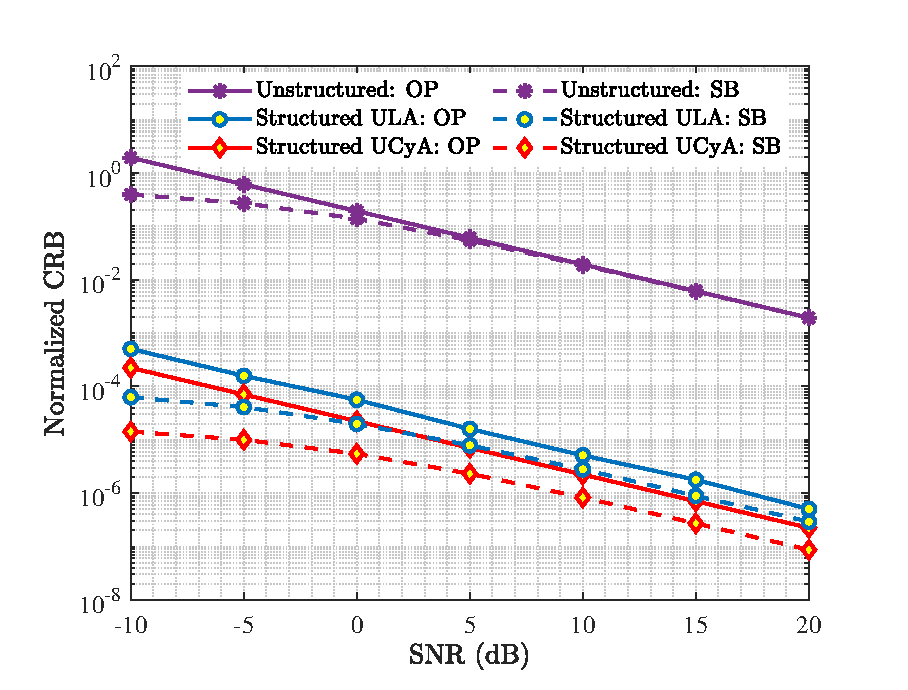
\includegraphics[width=\linewidth]{figures/fig_1_3.eps}
    \caption{CRB của hai cấu hình ULA và UCyA ứng với mô hình kênh truyền có cấu trúc (structured) và không sử dụng cấu trúc (unstructured). Cấu hình của mảng ăng-ten như sau $N_{ULA} = 96, N_{UCA} = 24,$ và $N_{3D} = 4$.}
    \label{fig:op}
\end{figure}

Trên hình~\ref{fig:op}, số lượng phần tử của mảng thu MIMO kích thước lớn là $96$ trong đó $N_{ULA}~=~96, N_{UCA} = 24,$ và $N_{3D} = 4$. Nhìn chung, sai số ước lượng của mô hình kênh truyền có cấu trúc vượt trội khi so sánh với mô hình kênh truyền không sử dụng cấu trúc với độ lợi khoảng $10^3$. Khi so sánh hai phương pháp ước lượng SB và OP, ở các mức SNR thấp (SNR $\le$ $5$~dB), phương pháp SB áp dụng cho mô hình kênh truyền không sử dụng cấu trúc có thể cho sai số thấp hơn một chút khi so sánh với việc chỉ sử dụng pilot của OP. Với mô hình kênh có cấu trúc, phương pháp SB vẫn cho CRB tốt hơn ở các mức SNR thấp, và giữ ở mức ổn định khi SNR $\ge 5$~dB. Tiếp đến là so sánh về ảnh hưởng của cấu hình mảng ăng-ten, cấu hình UCyA cho độ chính xác cao hơn so với ULA ở cả hai phương pháp ước lượng OP và SB. Có thể rút ra nhận xét, việc sử dụng mô hình kênh truyền có cấu trúc, phương pháp ước lượng SB, và cấu hình mảng ăng-ten 3D (UCyA) có thể cho ra độ chính xác cao hơn cho các bộ nhận dạng của hệ thống mMIMO.
\begin{figure}[ht]
    \centering
    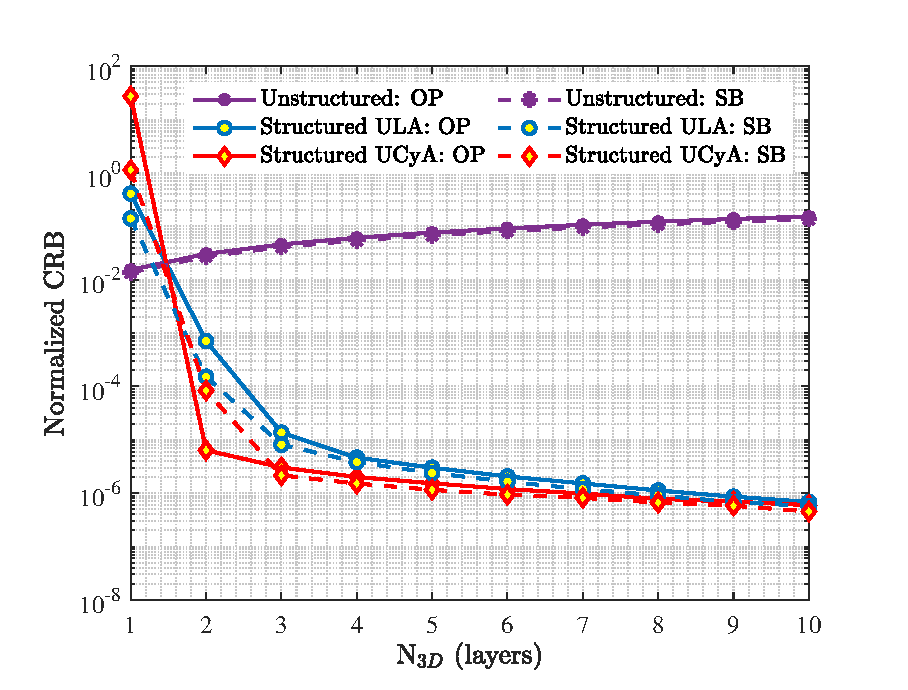
\includegraphics[width=\linewidth]{figures/fig_2_3.eps}
    \caption{CRB của hai cấu hình ULA và UCyA khi thay đổi $N_{3D}$. Các thông số mô phỏng như sau $N_{UCA} = 24, N_{ULA} = 24 * N_{3D}$, và SNR $=5$~dB.}
    \label{fig:op_N3D}
\end{figure}

Trên hình~\ref{fig:op_N3D}, số lượng các lớp $N_{3D}$ của cấu hình UCyA được khảo sát bằng cách giữ nguyên số phần tử thuộc mảng vòng $N_{UCA} = 24$ và SNR~$=5$~dB. Một lần nữa, các CRB chỉ ra rằng với $N_{3D}$ khác nhau, mô hình kênh truyền có cấu trúc hầu như có thể cho ra sai số ước lượng thấp hơn mô hình kênh truyền không sử dụng cấu trúc. Xét riêng mô hình kênh truyền không sử dụng cấu trúc, số $N_{3D}$ tăng lên kéo theo sai số ước lượng cũng tăng lên dù không quá lớn. Ngay cả khi sử dụng phương pháp ước lượng SB, độ chính xác thu được với mô hình kênh có cấu trúc cũng gần như không được cải thiện. Ngược lại, với mô hình kênh truyền có cấu trúc, CRB có xu hướng đi xuống khi số lớp của mảng UCyA tăng cho đến khi tất cả hội tụ tại sai số khoảng $10^{-6}$. Tại các giá trị $N_{3D}$ nhỏ, trong khoảng từ $2$ đến $6$ lớp, việc sử dụng cấu hình UCyA nhìn chung vẫn cho hiệu quả đáng kể so với ULA. Khi xem xét sự ảnh hưởng của phương pháp OP hay SB trong kịch bản này, rõ ràng không có sự khác biệt quá rõ ràng nếu $N_{3D} \ge 3$. Có thể rút ra nhận xét thứ hai, sử dụng mô hình kênh truyền có cấu trúc và cấu hình mảng UCyA có thể cho hiệu suất ước lượng kênh truyền tốt hơn khi $N_{3D}$ nhỏ. Tuy nhiên, lưu ý rằng, ngoài lợi thế về độ chính xác, khi số lượng phần tử trong mảng lên đến $240$ như trong mô phỏng, cấu hình mảng UCyA sẽ giúp tiết kiệm được rất nhiều diện tích lắp đặt mảng ăng-ten.
\begin{figure}[ht]
    \centering
    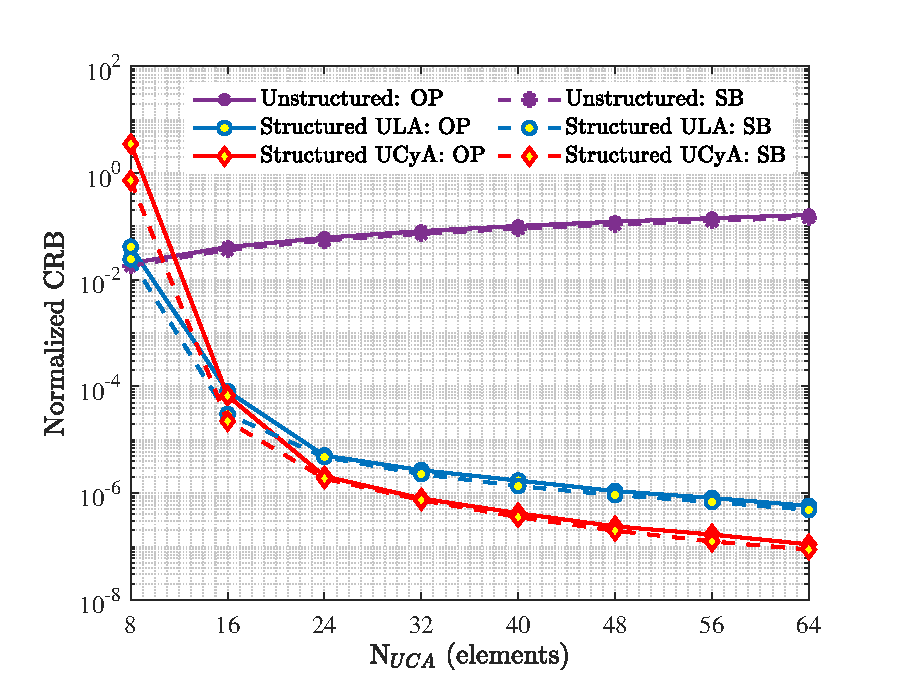
\includegraphics[width=\linewidth]{figures/fig_3_3.eps}
    \caption{CRB của hai cấu hình ULA và UCyA khi thay đổi $N_{UCA}$. Các thông số mô phỏng như sau $N_{3D} = 4, N_{ULA} = 4 * N_{UCA}$, và SNR $=5$~dB.}
    \label{fig:op_NUCA}
\end{figure}

Cuối cùng, trên hình~\ref{fig:op_NUCA}, số lượng phần tử của một mảng tròn UCA được thay đổi trong khoảng từ $8$ đến $64$ phần tử, trong khi giữ nguyên $N_{3D} = 4, N_{ULA} = 4 \times N_{UCA}$, và SNR $=5$~dB. Do CRB của mô hình kênh truyền không sử dụng cấu trúc chỉ bị ảnh hưởng bởi số lượng phần tử ăng-ten nên các CRB này vẫn giữ như trên hình~\ref{fig:op_N3D}. Với mô hình kênh truyền có cấu trúc, CRB thay vì hội tụ tại một điểm sẽ có xu hướng giảm dần cùng với $N_{UCA}$. Khi số phần tử $N_{UCA}$ đủ lớn ($N_{UCA} \ge 24$), các CRB của UCyA cho độ chính xác tốt hơn một cách tuyến tính khi so sánh với mảng ULA. Phương pháp SB trong kịch bản mô phỏng này nhìn chung chỉ cho độ chính xác tốt hơn nhưng không nhiều so với OP. Có thể rút ra nhận xét thứ ba, sử dụng mô hình kênh truyền có cấu trúc và cấu hình mảng UCyA có thể cho hiệu suất ước lượng kênh truyền tốt hơn và tăng dần với $N_{UCA}$. Tuy nhiên, cần lưu ý dù cho độ chính xác cao hơn, nhưng khi $N_{UCA}$ tăng cao, bán kính của mảng tròn UCA lớn dần lại dẫn đến lãng phí diện tích lắp đặt mảng ăng-ten.

\section{Kết luận chương}
Trong chương này, đường bao Cramér Rao đã được sử dụng để xem xét ảnh hưởng của các cấu hình mảng ăng-ten khác nhau đến sai số ước lượng kênh truyền trong các hệ thống mMIMO. Lý thuyết về CRB cho việc ước lượng kênh truyền được trình bày trong hai trường hợp, OP và SB. Các kết quả mô phỏng đã chỉ ra hiệu năng của việc ước lượng kênh truyền có thể được cải thiện rõ rệt nếu sử dụng mô hình kênh truyền có cấu trúc. Ngoài ra, cấu hình mảng ăng-ten UCyA và phương pháp SB cũng sẽ góp phần cải thiện độ chính xác khi so sánh với cấu hình ULA và phương pháp OP truyền thống.